\documentclass[12pt]{report}

\usepackage[letterpaper, hmargin=0.75in, vmargin=0.75in]{geometry}

\usepackage{
    courier,
    algorithm,
    algpseudocode,
    listings,
    underscore,
    authblk,
    hyperref,
    tikz,
    tabularx,
    float,
    graphicx,
	  color
}

\lstset{basicstyle=\footnotesize\ttfamily}

\setlength{\parindent}{0pt}

\begin{document}

\title{RTX Software Design Report}

\author{
    Clement Hoang\\
		20531116\\
    \texttt{c8hoang@uwaterloo.ca}
    \and
    David Su\\
		20516776\\
    \texttt{dysu@uwaterloo.ca}
    \and
    Cole Vander Veen\\
		20503626\\
    \texttt{cgvander@waterloo.ca}
    \and
    Peter Li\\
		20522308\\
    \texttt{y648li@uwaterloo.ca}
}

\date{Winter 2016}

\maketitle


\tableofcontents
\listofalgorithms
\listoffigures

\chapter{Introduction}

The purpose of this report is to outline the design of the RTX written by the group members, Clement Hoang, David Su, Peter Li, and Cole Vander Veen, as part of the SE350 course at the University of Waterloo. The OS is designed for a Keil MCB1700 Cortex-M3 board, with a LPC1768 microcontroller.

It is aimed to provide documentation for the operating system, in order to facilitate the use and understanding for anyone interested in programming for the OS. As such, this report outlines the global variables used in the OS, and then moves on to describing the kernel API in a modular and chronological way, from when we implemented it. Finally, the report closes with some analysis on the OS, and challenges that the group faced for the duration of the lab.

\chapter{Design Description}

\section{Global Variables and Data Structures}
\begin{itemize}
  \item \texttt{memQueue}: A data structure that models the free physical memory in the OS, by splitting the heap into blocks of equal size. It is represented by a \texttt{MemQueue} data structure, which is a linked list of \texttt{MemBlock} nodes of size \texttt{BLOCK_SIZE}. It is used by the kernel API when releasing and requesting memory, by popping a block when it is used by a process, and pushing it back in when it is released.
    \begin{itemize}
      \item \texttt{MemBlock}: To expand, the \texttt{MemBlock} is a C-struct that holds a pointer to the next \texttt{MemBlock} in the queue. It also has reserved space in the front in case the block needs to hold an \texttt{envelope}. The \texttt{envelope} contains the following fields:
        \begin{itemize}
          \item \texttt{next}: a pointer to the next envelope in the queue
          \item \texttt{sender_id}: the process ID of the sender
          \item \texttt{recv_id}: the process ID of the receiver
          \item \texttt{send_time}: the time it was originally sent at
        \end{itemize}
    \end{itemize}
  \item \texttt{gp_pcbs}: A pointer to an array of \texttt{PCB} structs. It holds the state of all the process control blocks that are in the OS, and is interacted with by functions that change and read PCB states. For example, setting the process priority or getting the process priority uses \texttt{gp_pcbs} to access the priority of a specific PCB.
    \begin{itemize}
      \item \texttt{PCB}: a model of a process and its state. The \texttt{PCB} contains the following fields:
        \begin{itemize}
          \item \texttt{mp_sp}: stack pointer of the process
          \item \texttt{m_pid}: ID of the process
          \item \texttt{m_priority}: priority of the process
          \item \texttt{m_state}: state of the process
          \item \texttt{nextPCB}: pointer to the next \texttt{PCB}, if it is in a queue
          \item \texttt{msgHead}: beginning of the message queue
          \item \texttt{msgTail}: end of the message queue
        \end{itemize}
    \end{itemize}
  \item \texttt{g_proc_table}: an array of \texttt{PROC_INIT} structs that contains process information for initialization. The \texttt{PROC_INIT} looks like the following:
    \begin{itemize}
      \item \texttt{m_id}: ID of the process
      \item \texttt{m_priority}: initial priority of the process
      \item \texttt{m_stack_size}: size to allocate for the process in words
    \end{itemize}
  The process table is used often during the \texttt{process_init()} function.
    \item \texttt{gp_stack}: a pointer to the top of the memory heap, which is also the last conceptual memory block in \texttt{memQueue}. It is used during \texttt{heap_init()}.
  \item \texttt{p_end}: a pointer to the beginning of the memory heap, which is also the first conceptual memory block in \texttt{memQueue}. It is calculated by starting at \texttt{\&Image\$\$RW_IRAM1\$\$ZI\$\$Limit}, then incrementing it upon PCB initialization in \texttt{memory_init()}.
  \item \texttt{numOfBlocks}: the number of blocks of \texttt{MemBlock} allocated in the \texttt{heap_init()}
  \item \texttt{g_switch_flag}: a boolean flag that indicates whether to continue to run the process before the UART receives an interrupt. If 1, then it will immediately switch, and if it's 0, then it will continue to run the process.
  \item \texttt{gp_current_process}: a pointer to the \texttt{PCB} of the currently running process. It is used in \texttt{process_switch()} among other functions that deal with the current process
  \item \texttt{ReadyPQ}: a linked list of linked lists of \texttt{PCB} structures. It represents a priority queue of process blocks in the ready queue. This is used for scheduling, for example inside the \texttt{scheduler()} function.
  \item \texttt{BlockPQ}: a linked list of linked lists of \texttt{PCB} structures. It represents a priority queue of process blocks in the blocked queue. This is used for scheduling, for example inside the \texttt{scheduler()} function.
  \item \texttt{NUM_OF_PRIORITIES}: a constant that represents the number of priorities in the OS (default = 5). 0-3 represent the normal priorities from highest to lowest, whereas 4 is the priority of the null process.
  \item \texttt{gp_buffer}: a pointer to the next location \texttt{g_buffer}. It is used in \texttt{c_UART0_IRQHandler()}.
  \item \texttt{g_buffer}: a circular buffer that keeps track of the input and wraps around at a certain size. It is used in \texttt{kcdProc()} and other functions that deal with uart input.
  \item \texttt{g_buffer_end}: a pointer to the last location in \texttt{g_buffer}. It is helpful for calculations in \texttt{kcdProc()}.
  \item \texttt{PROC_STATE_E}: An enum which consists of the states:
    \begin{itemize}
      \item \texttt{NEW}: process was just created
      \item \texttt{RDY}: process is on the ready queue
      \item \texttt{RUN}: process is currently running
      \item \texttt{BLK}: process is blocked on memory
      \item \texttt{WAIT}: process is waiting to receive a message
    \end{itemize}
  \item \texttt{MSG_BUF}: It represents a message buffer and is a part of an \texttt{envelope}, with some space in memory blocks reserved for it. It consists of the following fields:
    \begin{itemize}
      \item \texttt{mtype}: a user defined message type
      \item \texttt{mtext}: a \texttt{char} array which contains the body of the message
    \end{itemize}
\end{itemize}

\section{Memory Management}

\subsection{Memory Overview}

% The ‘heap’ that the processes request memory blocks from is maintained as a linked list. The length of the heap is exactly enough space for thirty memory blocks of size 0x80 (128 bytes). The number of memory blocks can be configured by modifying the NUM_BLOCKS constant.
% Free space nodes keep track of the length of free space following this address and a pointer to the next chunk of unclaimed blocks. These headers are written directly into the blocks as they are returned to the heap. They are free to be overwritten, the only safe header is the starting address of the heap. The heap is shifted by four bytes to protect the last block from ever being overwritten.
% The request and release methods maintain the optimal structure of the list, deleting and overwriting excess or useless nodes.

By keeping track of the \texttt{gp_stack} and \texttt{gp_pcbs} pointers and keeping track of how much memory the \texttt{PCB}s use, then it is possible to do some pointer arithmetic to determine the starting and ending addresses of the heap (the physical memory available to allocate in the RTX).

The implementation of memory management in this RTX involves maintaing a linked list that keeps track of all the available \texttt{MemBlock}s on the heap. Upon process consumption of memory, \texttt{MemBlock}s allocated are removed from the linked list and a reference to the block is kept in the process. Upon release, the \texttt{MemBlock} is appended to the linked list again. This has performance implications of $O(1)$ for deletion and insertion of blocks.

 The \texttt{MemBlock}s have a user-defined size called \texttt{BLOCK_SIZE}. The system also reserves some space in the beginning of \texttt{MemBlock}s for \texttt{envelope}s. By default, the \texttt{BLOCK_SIZE} is set to 128 bytes.

\begin{figure}[h!]
  \centering
	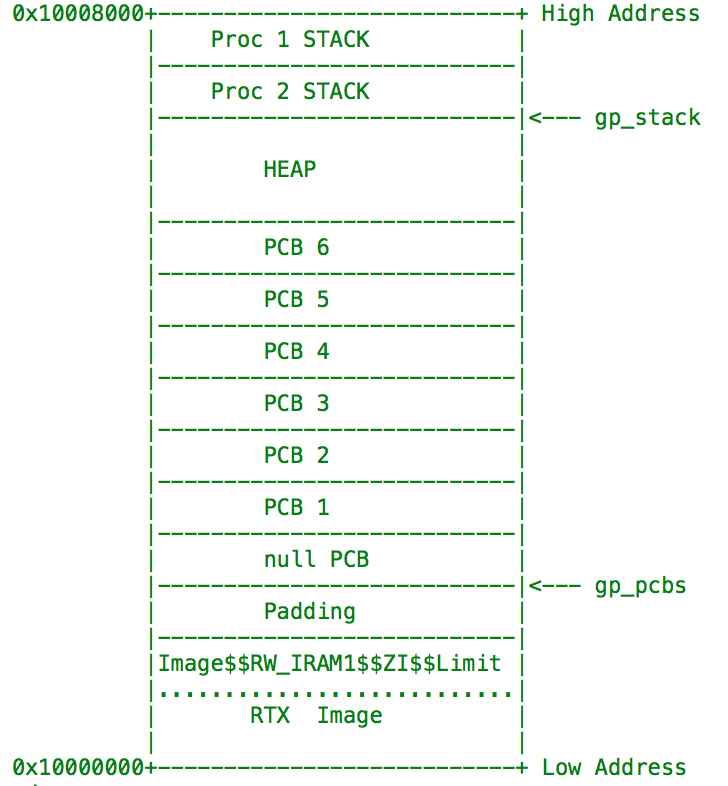
\includegraphics{memory.png}
\caption{Memory Layout}

\end{figure}

\subsection{Requesting Memory Blocks}

\begin{minipage}{\textwidth}
\begin{lstlisting}[language=C, frame=single]
int k_request_memory_block(void);
\end{lstlisting}
\end{minipage}

This function doesn't take any parameters, and returns the address of an available \texttt{MemBlock}. The algorithm is basically a queue dequeue function. It takes the previous head of \texttt{memQueue}, returns it, then updates the linked list accordingly.

\begin{algorithm}[H]
  \caption{Requesting memory function}
  \begin{algorithmic}[1]
    \Procedure{request\_memory\_block}{}
      \While{heap is full}
			\State {block the current process}
	  \EndWhile
	  \State {update the free space list}
	  \State {return the address of the top of the block}
    \EndProcedure
  \end{algorithmic}
\end{algorithm}

\subsection{Releasing Memory Blocks}

\begin{minipage}{\textwidth}
\begin{lstlisting}[language=C, frame=single]
int k_release_memory_block(void* memory_block);
\end{lstlisting}
\end{minipage}

This function takes a \texttt{MemBlock} parameter. This parameter is a reference to the \texttt{MemBlock} that will be freed. It also returns a flag on whether that operation was a success or not - \texttt{RTX_ERR} or \texttt{RTX_OK}. The algorithm is basically a queue enqueue function. After some validation logic, it attached the freed memory block to the end of the linked list. It also moves processes into the ready queue if possible.

\begin{algorithm}[H]
  \caption{Releasing memory function}
  \begin{algorithmic}[1]
    \Procedure{release\_memory\_block}{*memory_block}
      \If{this block is the top block of the heap}
			\State {modify heap header node (never gets overwritten)}
	  \EndIf
	  \If{there is free space immediately beneath this block}
			\State {combine them by increasing this block's length}
	  \Else { this block becomes a new block node, is added to the list}
	  \EndIf
	  \If{there is free space immediately beneath this block}
			\State {combine them by increasing this block's length}
	  \EndIf
	  \If{a process is blocked on memory}
			\State {unblock that process, release the processor}
	  \EndIf
    \EndProcedure
  \end{algorithmic}
\end{algorithm}

\pagebreak


%%%%%%%%%%%%%%%%%%%%%%%%%%%%%%%%%%%%%%%%%%%%%%%%%%%%%%%%%%%%%

\section{Processor Management}

\subsection{Process Control Structures}
awefawef

\subsection{Process Queues}
awefawef

\subsection{Process Scheduling}
sdfasdfasdfdasf

%%%%%%%%%%%%%%%%%%%%%%%%%%%%%%%%%%%%%%%%%%%%%%%%%%%%%%%%%%%%%

\section{Process Priority Management}

\subsection{Get Process Priority}

The get process priority function takes in the process id as a parameter and returns its priority. We denote the priority of -1 if the process is not found. To find the process by its id, we loop through all the pcbs which are stored in gp_pcbs and compare the process_id. If a matching pcb is found, then we retrieve its priority and return. Otherwise, the loop will end without ever finding a process and will -1.

\begin{algorithm}[H]
  \caption{Get Process Priority}
  \begin{algorithmic}[1]
  \Function {k_get_process_priority}{process_id}
  \State int priority = -1;
  \For {every process in pcb array}
    \If {process found}
      \State priority = process.priority;
      \State return priority;
     \EndIf
  \EndFor
  \State return priority;
  \EndFunction
  \end{algorithmic}
\end{algorithm}

\subsection{Set Process Priority}

The set process priority function takes in the process id and a priority as the parameters and returns if the function has completed successfully. First we loop through all the process ids to see if we can find a process that has matching ids. Then if we have found the process, we check to see if the priority that is being set to is different from the priority it's currently at. Now at this stage we store the old priority and set the new one if its not currently executing, otherwise we would undo the priority change if the priority change would somehow fail. Finally, we release the processor since we need to immediately move the higher priority process because of the change.

\begin{algorithm}[H]
  \caption{Set Process Priority}
  \begin{algorithmic}[1]
  \Function {k_set_process_priority}{int process_id, int priority}
    \If {priority is within valid range}
      \For {every user process}
        \If {process found}
          \If {process.priority is different}
            \State old_priority = process.priority;
            \State process.priority = priority;
            \If {process is not currently executing}
              \State attempt move the process priority, else undo priority
            \EndIf     
            \State release the processor
          \EndIf
        \EndIf
      \EndFor
    \EndIf
  \EndFunction
  \end{algorithmic}
\end{algorithm}

%%%%%%%%%%%%%%%%%%%%%%%%%%%%%%%%%%%%%%%%%%%%%%%%%%%%%%%%%%%%%

\section{Interprocess Communication}

\subsection{Message Structure}

Every message uses a memory block as its underlying storage component, and has 2 parts: the part visible to the user (the struct \texttt{MSG_BUF}), and the part exclusive to the kernel (the struct \texttt{envelope}). 

Every memory block created in the operating system has the first \texttt{sizeof(envelope)} bytes reserved, in case that memory block is used as a message. The envelope stores metadata about the message, such as the sender, receiver, the send time, etc. 

Every process' PCB has a ``mailbox'', with a linked list of messages sent to that process that have not yet been read. Thus, the envelope also has a pointer pointing to the next envelope in that linked list.

Then, there is the \texttt{MSG_BUF} struct, which is directly accessible by the user processes. The \texttt{MSG_BUF} contains 2 pieces of data: the type of the message (often \texttt{\#defined} as a constant), and the actual body of the message. The body of the message can take up the rest of the memory block (i.e. BLOCK_SIZE - sizeof(envelope) - sizeof(MSG_BUF.mtype)). 


\subsection{Sending Messages}

The send message primitive receives as parameters the intended recipient of the message, and a pointer to the memory block with the actual message. First, a few pieces of metadata is set on the envelope. Then, it merely places that message in the mailbox, located in the PCB of the recipient. Finally, if that message is blocked waiting for a message, it puts that message on the ready queue. Additionally, if that message has higher priority than the current running process, it releases the processor.

\begin{algorithm}[H]
	\caption{Send Message}
	\begin{algorithmic}[1]
		\Function{send_message}{receiver_id, message}
			\State message.sender = current process
			\State message.receiver = receiver_id
			\State enqueue message in the the receiver's mailbox
			\If{receiver was blocked waiting for a message}
				\State put receiver on the ready queue
				\State set receiver's state to Ready
				\If{receiver has higher priority than the current process}
					\State release the processor
				\EndIf
			\EndIf
		\EndFunction
	\end{algorithmic}
\end{algorithm}

In addition to the \texttt{send_message()} function specified above, we needed another version of the function that would not preempt under any circumstances. This was necessary for the case when the UART i-process needed to send a message. I-processes must not preempt under any circumstances.

\begin{algorithm}[H]
	\caption{Send Message (Non-preemptive)}
	\begin{algorithmic}[1]
		\Function{send_message_non_preempt}{receiver_id, message}
			\State message.sender = current process
			\State message.receiver = receiver_id
			\State enqueue message in the the receiver's mailbox
			\If{receiver was blocked waiting for a message}
				\State put receiver on the ready queue
				\State set receiver's state to Ready
			\EndIf
		\EndFunction
	\end{algorithmic}
\end{algorithm}


Finally, we created another version of \texttt{send_message()} specific to the timer i-process. The timer i-process must send messages to other processes once the timeout expires. However, the sender of that message is not the timer i-process, but rather the original sender. Thus, this necessitated the creation of a new function. Again, this version is non-preemptive for the same reasons as \texttt{send_message_non_preempt()}.

\begin{algorithm}[H]
	\caption{Send Message (Timer version)}
	\begin{algorithmic}[1]
		\Function{timer_send_message}{message}
			\State receiver = message.receiver
			\State enqueue message in the the receiver's mailbox
			\If{receiver was blocked waiting for a message}
				\State put receiver on the ready queue
				\State set receiver's state to Ready
			\EndIf
		\EndFunction
	\end{algorithmic}
\end{algorithm}

\subsection{Receiving Messages}

Receive message merely involves checking the current running process' mailbox, and seeing if there is any messages there. If there is, deque that message, and return it immediately. Otherwise, set the current process' state to blocked on receive, and release the processor.

\begin{algorithm}[H]
	\caption{Receive Message}
	\begin{algorithmic}[1]
		\Function{receive_message}{}
			\While{there are no messages in the current process' mailbox}
				\State current_process.state = BLOCKED_ON_RECEIVE
				\State release the processor
			\EndWhile

			\State dequeue the first message in the mailbox
			\State\Return message, sender_id
		\EndFunction
	\end{algorithmic}
\end{algorithm}

Similar to sending messages, receiving messages also needs a non_blocking version, to be used by the i-processes. If there are no messages in an i-process' mailbox, it should never block. Instead, it should return immediately, and indicate that there are no messages. This function is mainly used by the timer i-process.

\begin{algorithm}[H]
	\caption{Receive Message (non-blocking)}
	\begin{algorithmic}[1]
		\Function{receive_message_non_blocking}{process}
			\If{there are no messages in the process' mailbox}
				\State\Return NULL
			\EndIf

			\State dequeue the first message in the mailbox
			\State\Return message, sender_id
		\EndFunction
	\end{algorithmic}
\end{algorithm}


\subsection{Delayed Send}

Delayed send is implemented by sending a message to the timer i-process specifying the time when the message should actually be sent to the intended recipient.

\begin{algorithm}[H]
	\caption{Delayed Send}
	\begin{algorithmic}[1]
		\Function{delayed_send}{receiver, message, delay}
			\State message.sender = current process
			\State message.receiver = receiver
			\State message.send_time = current_time + delay

			\State enqueue the message in the timer i-process's mailbox 
		\EndFunction
	\end{algorithmic}
\end{algorithm}

%%%%%%%%%%%%%%%%%%%%%%%%%%%%%%%%%%%%%%%%%%%%%%%%%%%%%%%%%%%%%

\section{Interrupts and I-Processes}

\subsection{UART I-Process}

The UART interrupt is enabled to send output to a display, and to receive input from the user. The OS handles those interrupts by registering a \texttt{UART0_IRQHandler} function that will be called whenever a UART interrupt occurs.

The file \texttt{uart_irq.c} is initialized by calling the function \texttt{uart_irq_init}. This function initializes the UART interrupts by setting the appropriate flags and choosing the correct UART port.

Below is the interrupt handling pseudocode, starting with UART0_IRQHandler:
\begin{algorithm}[H]
	\caption{UART Interrupt Handler function (assembly)}
	\begin{algorithmic}[1]
	  \Function{UART0_IRQHandler}{}
	    \State push registers onto stack
	    \State call c_UART0_IRQHandler_wrapper()
	    \State pop registers off stack
	  \EndFunction
	\end{algorithmic}
\end{algorithm}

\begin{algorithm}[H]
	\caption{UART Interrupt Handler function wrapper (C)}
	\begin{algorithmic}[1]
	  \Function{c_UART0_IRQHandler_wrapper}{}
	    \State call c_UART0_IRQHandler()
	    \If{there is another ready process with higher priority than the current process}
	      \State call k_release_processor()
	    \EndIf
	  \EndFunction
	\end{algorithmic}
\end{algorithm}

\begin{algorithm}[H]
	\caption{Main UART Interrupt Handler function (C)}
	\begin{algorithmic}[1]
	  \Function{c_UART0_IRQHandler}{}
	    \If{receive data available}
	      \State g_char_in = newly received char
	      \If{g_char_in == null character}
	        \State\Return
	      \EndIf

	      \State echoMsg = get memory block (non blocking)
	      \If{echoMsg is not null}
	        \State echoMsg-$>$mtype = ECHO
	        \If{g_char_in == '\textbackslash r'}
	          \State echoMsg-$>$mtext = \verb|"\n\r\0"|
	        \Else
	          \State echoMsg-$>$mtext = g_char_in + \verb|'\0'|
	        \EndIf
	        \State send echoMsg (no preemption) to KCD
	      \EndIf
	      \If{cur_msg is null}
	        \State cur_msg = get memory block (non blocking)
	        \If{cur_msg is null (no more memory)}
	          \State\Return
	        \EndIf

	        \State msg_str_index = 0
	      \EndIf

	      \If{g_char_in == '\textbackslash r' or message about to overflow memory block}
	        \State cur_msg-$>$mtext += '\textbackslash 0'
	        \State cur_msg-$>$mtype = DEFAULT
	        \State send cur_msg (no preemption) to KCD
	        \State reset cur_msg, msg_str_index
	      \Else
	        \State cur_msg-$>$mtext += g_char_in
	      \EndIf
	    \ElsIf{transmit interrupt enabled}
	      \If{*gp_buffer != null character}
	        \State send *gp_buffer
	        \State gp_buffer = next location in circular buffer
	      \Else
	        \State disable transmit interrupt
	        \State send null character
	        \State reset gp_buffer and g_buffer_end
	      \EndIf
	    \EndIf
	  \EndFunction
	\end{algorithmic}
\end{algorithm}

If there is an incoming character, immediately forward it to the KCD (assuming there is free memory) to echo back to the user. Also, add that character to a buffer. Once a newline is encountered, send the entire buffer to the KCD to decode

If there are still messages in the transmit buffer, send the next character. If the character is a null character, disable the transmit interrupt as the transmission is finished.


Also, there is an \texttt{enable_UART_transmit()} function that sets the appropriate flags to enable the interrupt for outputting characters. This function is called by the CRT to begin outputting characters.


\subsection{Timer I-Process}

sdfasfdafd

%%%%%%%%%%%%%%%%%%%%%%%%%%%%%%%%%%%%%%%%%%%%%%%%%%%%%%%%%%%%

\section{System Processes}

\subsection{Null Process}

The null process simply releases the processor in an infinite loop.

\begin{algorithm}[H]
	\caption{Null Process}
	\begin{algorithmic}[1]
		\Function{nullProc}{}
			\While{true}
				\State k_release_processor()
			\EndWhile
		\EndFunction		
	\end{algorithmic}
\end{algorithm}

\subsection{CRT Process}

The CRT's sole responsibility is to output the contents of the messages they receive to the UART.

\begin{algorithm}[H]
	\caption{CRT Process}
	\begin{algorithmic}[1]
	  \Function{crtProc}{}
	    \While{true}
	      \State msg = receive\_message()
	      \State copy msg-$>$mtext to output buffer
	      \State enable\_UART\_transmit()
	      \State release\_memory\_block(msg)
	    \EndWhile
	  \EndFunction
	\end{algorithmic}
\end{algorithm}

\begin{algorithm}[H]
	\caption{Copy string to circular buffer helper function}
	\begin{algorithmic}[1]
	  \Function{copyToBuffer}{str}
	    \For{each char in str}
	      \State g_buffer[g_buffer_end] = char
	      \State g_buffer_end = (g_buffer_end + 1) mod BUFFER_SIZE
	    \EndFor
	  \EndFunction
	\end{algorithmic}
\end{algorithm}

\subsection{KCD Process}

The KCD's (Keyboard Command Decoder) responsibility is to decode messages that it receives, and forward them to the appropriate process that has registered itself to handle these types of messages.

\begin{algorithm}[H]
	\caption{KCD Process}
	\begin{algorithmic}[1]
	  \Function{kcdProc}{}
	    \State identifiers = empty array
	    \State processes = empty array
	    \State numIdentifiers = 0
	    \While{true}
	      \State msg = receive\_message()
	      \If{msg-$>$mtype == KCD\_REG}
	        \State add msg's identifier to identifiers
	        \State add msg's sender to processes
	        \State numIdentifiers++
	        \State release\_message\_block(msg)
	      \ElsIf{msg-$>$mtype == ECHO}
	        \State send\_message(PID\_CRT, msg)
	      \Else
	        \If{msg-$>$mtext starts with '\%'}
	          \State handler = search for handler in identifiers
	        \EndIf
	        \If{no handler for this type of message}
	          \State release\_memory\_block(msg)
	        \Else
	          \State send\_message(handler, msg)
	        \EndIf

	        \If{msg-$>$mtext begins with '!'}
	          \State search through PCBs for processes in ready state
	          \State debugMsg = create message with those processes
	          \State send\_message(PID\_CRT, debugMsg)
	        \ElsIf{msg-$>$mtext begins with '@'}
	          \State search through PCBs for processes in blocked state
	          \State debugMsg = create message with those processes
	          \State send\_message(PID\_CRT, debugMsg)
	        \ElsIf{msg-$>$mtext begins with '\#'}
	          \State search through PCBs for processes in blocked on message state
	          \State debugMsg = create message with those processes
	          \State send\_message(PID\_CRT, debugMsg)
	        \EndIf
	      \EndIf
	    \EndWhile
	  \EndFunction
	\end{algorithmic}
\end{algorithm}

This processes repeatedly receives messages. If it is a keyboard command registration, the process saves the identifier along with the process that is registered to handle those commands. If it is an echo command, the message is merely forwarded to the CRT. Otherwise, if the message is an actual command (i.e. it starts with a '\%'), the message is forwarded to the process that is registered to handle it, if it exists. Finally, if the message begins with any debug hotkey, the corresponding debug output is sent to the CRT.

%%%%%%%%%%%%%%%%%%%%%%%%%%%%%%%%%%%%%%%%%%%%%%%%%%%%%%%%%%%%%

\section{User Processes}

\subsection{Wall Clock Process}

This process receives messages to reset, start at a specified time, and stop the wall clock. Once started, the clock will print the elapsed time every second.

\begin{algorithm}[H]
	\caption{Wall Clock Process}
	\begin{algorithmic}[1]
	  \Function{wallClockProc}{}
	    \State register itself with KCD to handle '\%W' commands
	    \State id = 0
	    \While{true}\texttt{}
	      \State msg = receive\_message()
	      \If{msg contains reset command}
	        \State id++
	        \State time = 0
	        \State send increment time command to itself, delayed 1 second
	        \State construct time string, send to CRT to print
	      \ElsIf{msg contains increment command}
	        \If{msg's id == id}
	          \State time++
	          \State send increment time command to itself, delayed 1 second
	          \State construct time string, send to CRT to print
	        \Else
	          \State release\_memory\_block(msg)
	        \EndIf
	      \ElsIf{msg contains a start at specified time command}
	        \State id++
	        \State time = parseTime(msg)
	        \State send increment time command to itself, delayed 1 second
	        \State construct time string, send to CRT to print
	      \ElsIf{msg contains stop command}
	        \State id++
	        \State release\_memory\_block(msg)
	      \Else
	        \State release\_memory\_block(msg)
	      \EndIf
	    \EndWhile
	  \EndFunction
	\end{algorithmic}
\end{algorithm}

\subsection{Set Priority Process}

This process registers itself with the KCD to handle ``\%C'' commands. It accepts as parameters a process id, and the new priority for that process.

\begin{algorithm}[H]
	\caption{Set Priority Process}
	\begin{algorithmic}[1]
	  \Function{setPriorityProc}{}
	  	\State send message to KCD to register itself to handle ``\%C'' commands

	  	\While{true}
	  		\State msg = receive new message
	  		\State parse msg's string to get the process_id and new priority to change to
	  		\If{error parsing string}
	  			\State print error message
	  			\State \textbf{continue}
	  		\EndIf

	  		\State set_process_priority(process_id, new_priority)
	  		\If{set_process_priority returned error code}
	  			\State print error message
	  		\EndIf
	  	\EndWhile
	  \EndFunction
	\end{algorithmic}
\end{algorithm}


% David - I don't think it's necessary to talk about stress tests
% \subsection{Stress Test Processes}
% dfdasfasdfads

\section{Initialization}

dasfasfasfd

\section{Testing}

dfadsfasdf

\section{Major Design Changes}

dsfdafadsf

\chapter{Lessons Learned}

Upon the completion of this project, the group has gained many valuable insights. This includes things like code quality, source control, and team dynamics.

\section{Version Control}
For our codebase, we used Git as version control. At first, it was a bit painful because we were mostly committing to the master branch and we haven't found out which files to add to the .gitignore yet. This led to a lot of merge conflicts from differing binary files.
However, when the project was in a more stable state, we later progressed to branching out for different tasks and modules. This proved to be quite helpful because it allowed us to separate concerns and work on tasks indepdently.
One way we could have improved this is by having a systematic review process. Because of the team's lack of periodic code reviews and the fact that we divided the work up, the team did not have the opportunity to learn about work that other team members worked on, resulting in a team whose knowledge was extremely speciaized and exclusive for each individual member. This meant that bugs relating to a certain module can only be understood by some members of the team, which sometimes slowed progress down. To improve on this, the team could have periodic code reviews to keep everyone up to date and knowledgable in all parts of the codebase.

\section{Code Management}
When the group first started off coding, the code was extremely unmodular, files were monolithic, comments were lacking, and globals were overly used. This made the code quite messy to look at, and as we progressed through the different parts of the lab, we found it increasingly difficult to debug and navigate through our codebase. Somewhere between P2 and P3, we hit a wall where our RTX had some fundamental bugs with regard to scheduling. However, it was very hard to trace this bug down with our style of code. We dedicated a few days to refactoring the code base; we added comments on hard to understand expressions, we tried to reduce the use of global variables if they were not needed, and we separated long functions into smaller re-usable components. The end result was that unit testing was a lot easier.

\section{Logging and Output}
For some memory issues, it was extremely hard to debug. Even when tracing through the debugger, looking at pointer values is not always the most intuitive. In order to make development easier, we decided to add scoped debug flags in our RTX in order to trace bugs without convoluting the output. For example, we had a \texttt{MEM_DEBUG} flag which could be enabled to output the available amount of memory blocks after each transaction in order to debug a memory leak, and have the default \texttt{DEBUG} flag enabled for less specialized debugging. This allowed us to more intuitively track errors down.

\chapter{Team Dynamics and Individual Responsibilities}
The team members did not enforce a strict task allocation process for deciding each members' responsibilities. Generally however, the scheduling process is similar to the following scenario:
Upon the initial lab introduction, all four of the members would be present, in order to discuss the material and areas of interest. Then, the members would split into two pairs to work on the parts they chose respectively, using pair programming concepts, and communication both online and offline. If one pair is finished earlier than the other, then they would usually group up with the remaining pair to work through the problem. Otherwise, they would colloratively merge the parts they've worked on into a final workiing product before the deadline.

\chapter{Timing Analysis}

\end{document}
